\subsubsection*{Zadanie~1.1.}
\begin{figure}[H]
    \centering
    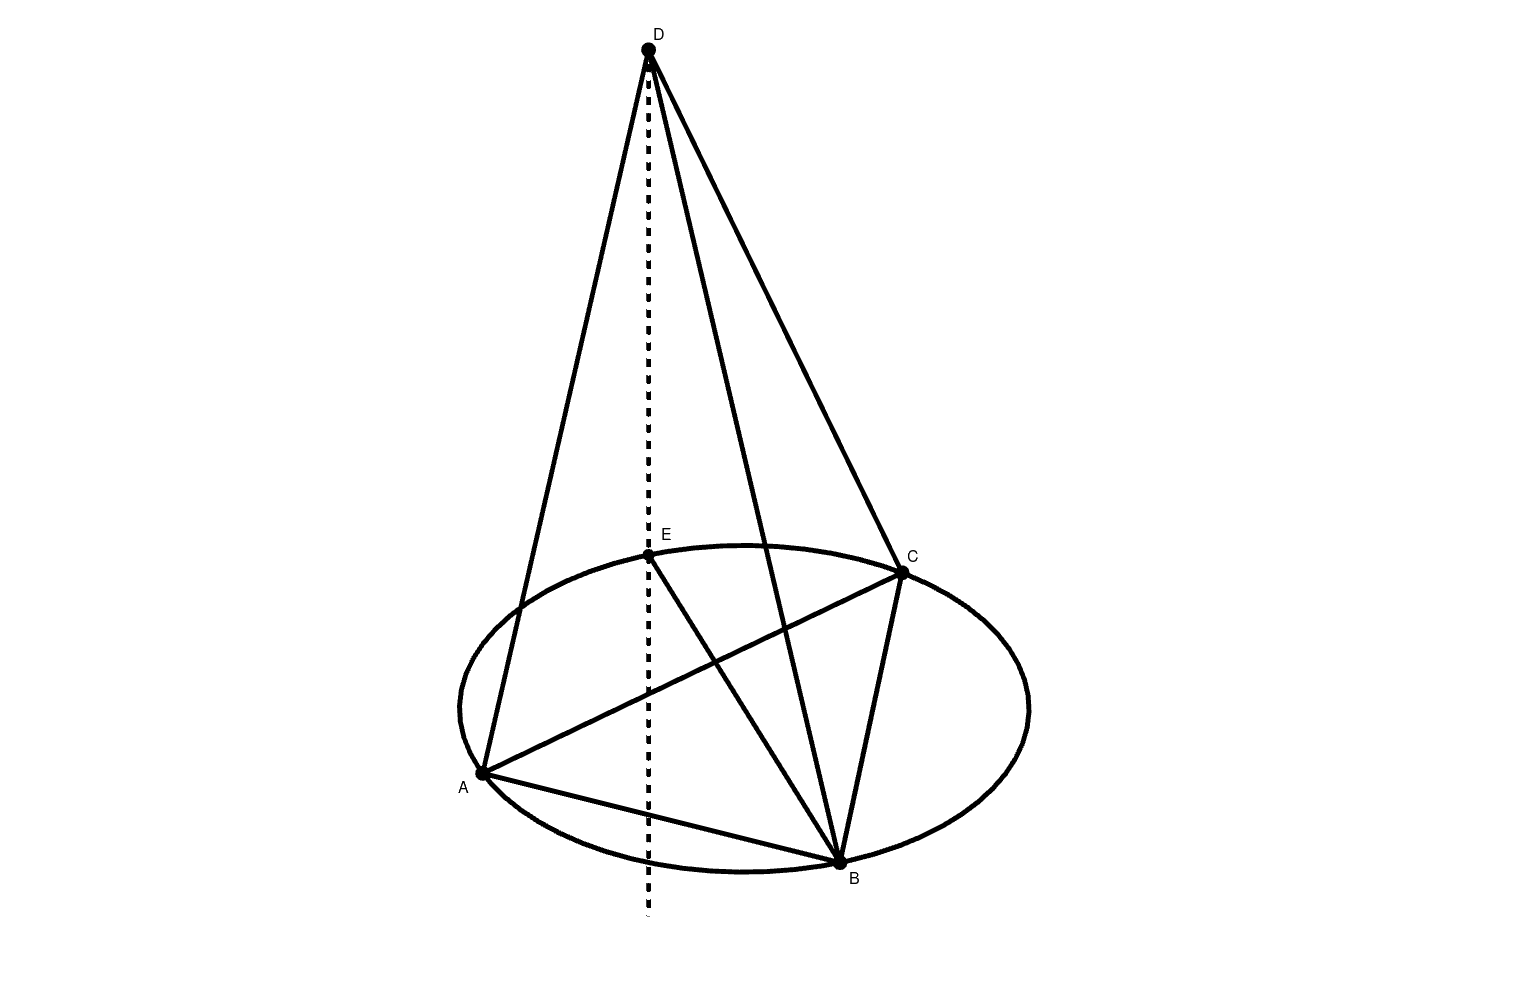
\includegraphics[width=\textwidth]{img/2021_01_27/1.png}
\end{figure}
Zauważmy, że skoro \(E\) jest spodkiem wysokości tego czworościanu, to prosta \(CE\) jest rzutem prostej \(CD\) na płaszczyznę podstawy. Ponieważ kąt \(\mangle{BCE}\) jest oparty na średnicy\(BE\) okręgu opisanego na \(\triangle{ABC}\), to \(CE \perp CB\). Z~twierdzenia o~trzech prostych prostopadłych wiemy natomiast, że jeśli rzut prostej na płaszczyznę jest prostopadły do pewnej innej prostej leżącej w~tej płaszczyźnie, to ta inna prosta jest prostopadła do prostej rzutowanej. Zatem \(CB \perp CD\). Analogicznie dowodzimy dla kąta \(\angle{DAB}\).
\qed
\subsubsection*{Zadanie~1.2.}
\begin{figure}[H]
    \centering
    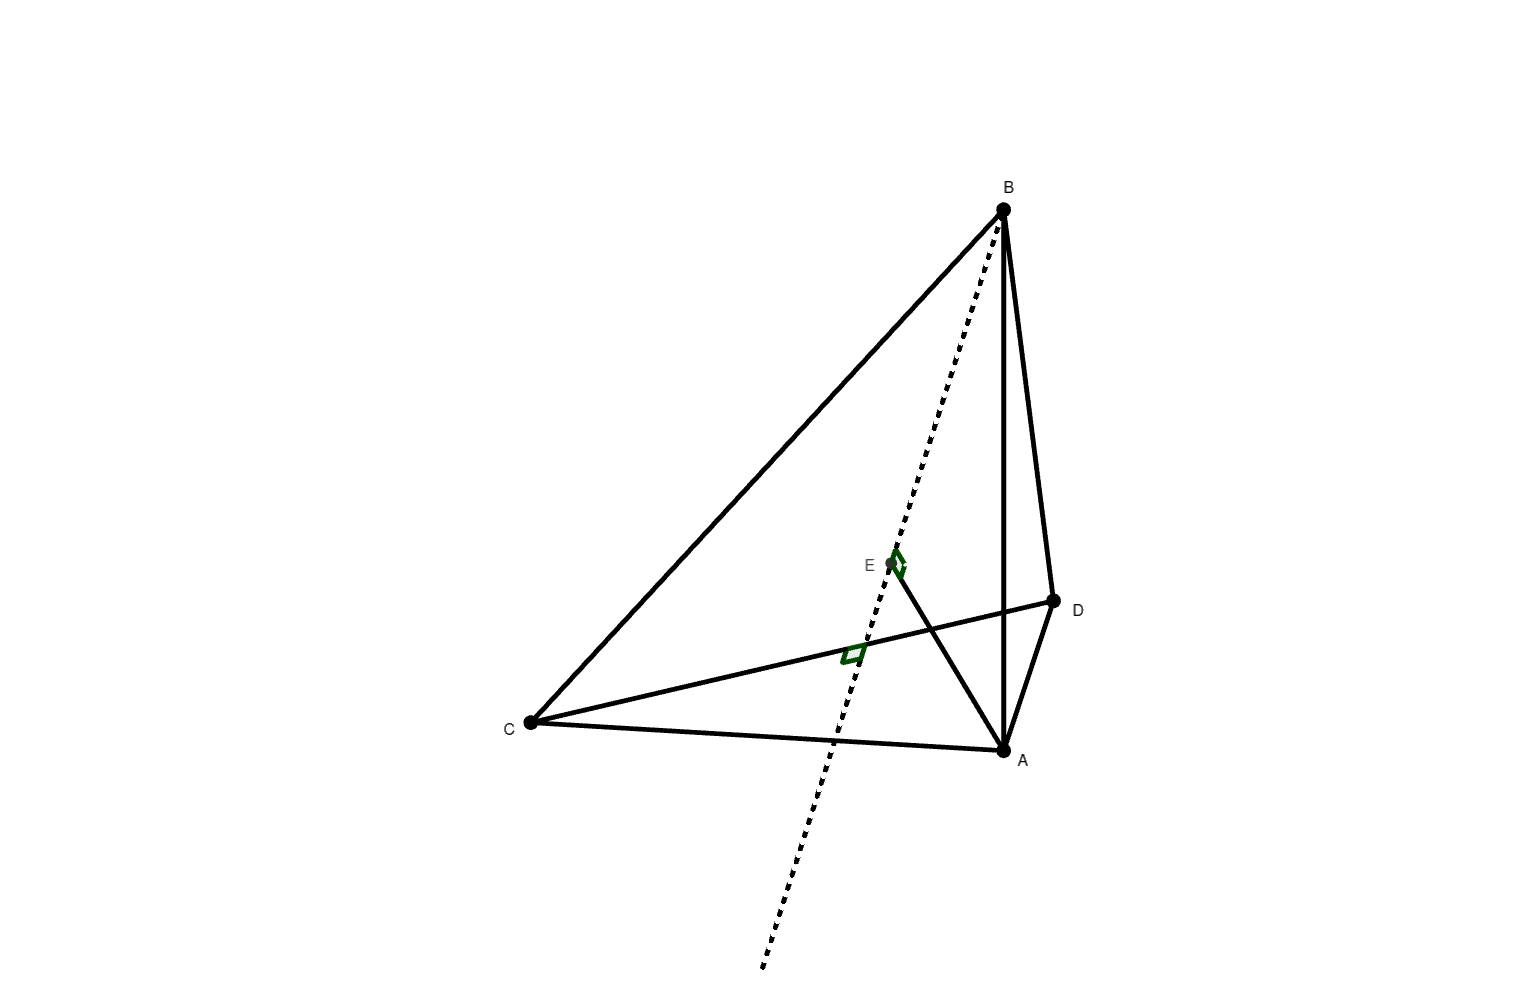
\includegraphics[width=\textwidth]{img/2021_01_27/2.png}
\end{figure}
Jeśli postawimy ten czworościan na ścianie \(ADC\), to \(BA\) będzie wysokością, ponieważ tak naprawdę tworzymy układ współrzędnych o~początku w~\(A\). Wtedy prosta \(AC\) będzie rzutem prostej \(BC\) na płaszczyznę \(ADC\). Wiemy natomiast, że \(AD \perp AC\), więc z~twierdzenia o~trzech prostych prostopadłych \(AD \perp BC\). Opuśćmy wysokość z~wierzchołka \(A\). Oznaczmy jej spodek na płaszczyźnie \(BCD\) przez \(E\). Wtedy \(DE\) jest rzutem prostej \(AD\) na płaszczyznę \(BCD\). Skoro wiemy, że \(BC\) jest prostopadła do \(AD\), to z~twierdzenia o~trzech prostych jest też prostopadła do jej rzutu, czyli \(BC \perp DE\), a~to oznacza, że \(DE\) jest wysokością w~\(\triangle{BCD}\). Analogicznie dowodzimy, że proste \(CE\) i~\(BE\) także są wysokościami tego trójkąta, pokazując tym samym, że \(E\) jest jego ortocentrum.
\qed

